\documentclass[11pt, a4paper]{article}
\usepackage[utf8]{inputenc}
% \usepackage{helvet}
\usepackage{graphicx}

% change default font family from serif to sans-serif
\renewcommand{\familydefault}{\sfdefault}
% change ToC, figure and table section titles to german equivalents
\renewcommand{\contentsname}{Inhaltsverzeichnis}
\renewcommand{\listfigurename}{Figuren- \& Abbildungsverzeichnis}
\renewcommand{\listtablename}{Tabellenverzeichnis}

\title{Projekttitel}
\date{2019-03-05}
\author{Projektdokumentation\\
       \\
       John Doe\\
       Awesome Denki - SuperElektrik GmbH\\
}

\begin{document}
  \pagenumbering{gobble}
  \maketitle
  \newpage

  \tableofcontents
  \newpage


  \pagenumbering{arabic}
  \section{Definitionsphase}
    \begin{abstract}
    Short introduction to subject of the paper \ldots
    \end{abstract}
    \subsection{Situationsanalyse}
    \subsection{Auftragsbeschreibung}
    \subsection{Problemdefinition}
    \subsection{Kundengespraech}
    \subsection{Ist-Analyse}
    \subsection{Soll-Konzept}
    \newpage

  \section{Planungsphase}
    \subsection{Projektstrukturplan}
    \subsection{Zeitplan}
    \subsection{Kostenplan}
    \subsection{Qualitaetssicherungsplan}
    \newpage

  \section{Durchfuehrungsphase}
    \subsection{Use Cases}
    \subsection{Domain Modelling}
    \subsection{Datenbankentwurf}
    \subsection{GUI-Entwurf}
    \newpage

  \section{Implementierungsphase}
    \subsection{Tests}
      \subsubsection{Unit Tests}
      \subsubsection{Systemtests}
      \subsubsection{Bedienungstests}
    \subsection{Quellcode}
    \subsection{Fachlicher Soll-Ist Vergleich}
    \subsection{Zeitlicher Soll-Ist Vergleich}
    \subsection{Installation \& Konfiguration???}
    \newpage

    \pagenumbering{gobble}
    \begin{appendix}
      \listoffigures
      \listoftables
    \end{appendix}
    \newpage

  \section{Anhang: Figuren \& Tabellen}
    \pagenumbering{Roman}
    \subsection{Fragenkatalog zum Kundengespraech}
      \newpage
    \subsection{Projektstrukturplan}
      \begin{figure}[h!]
        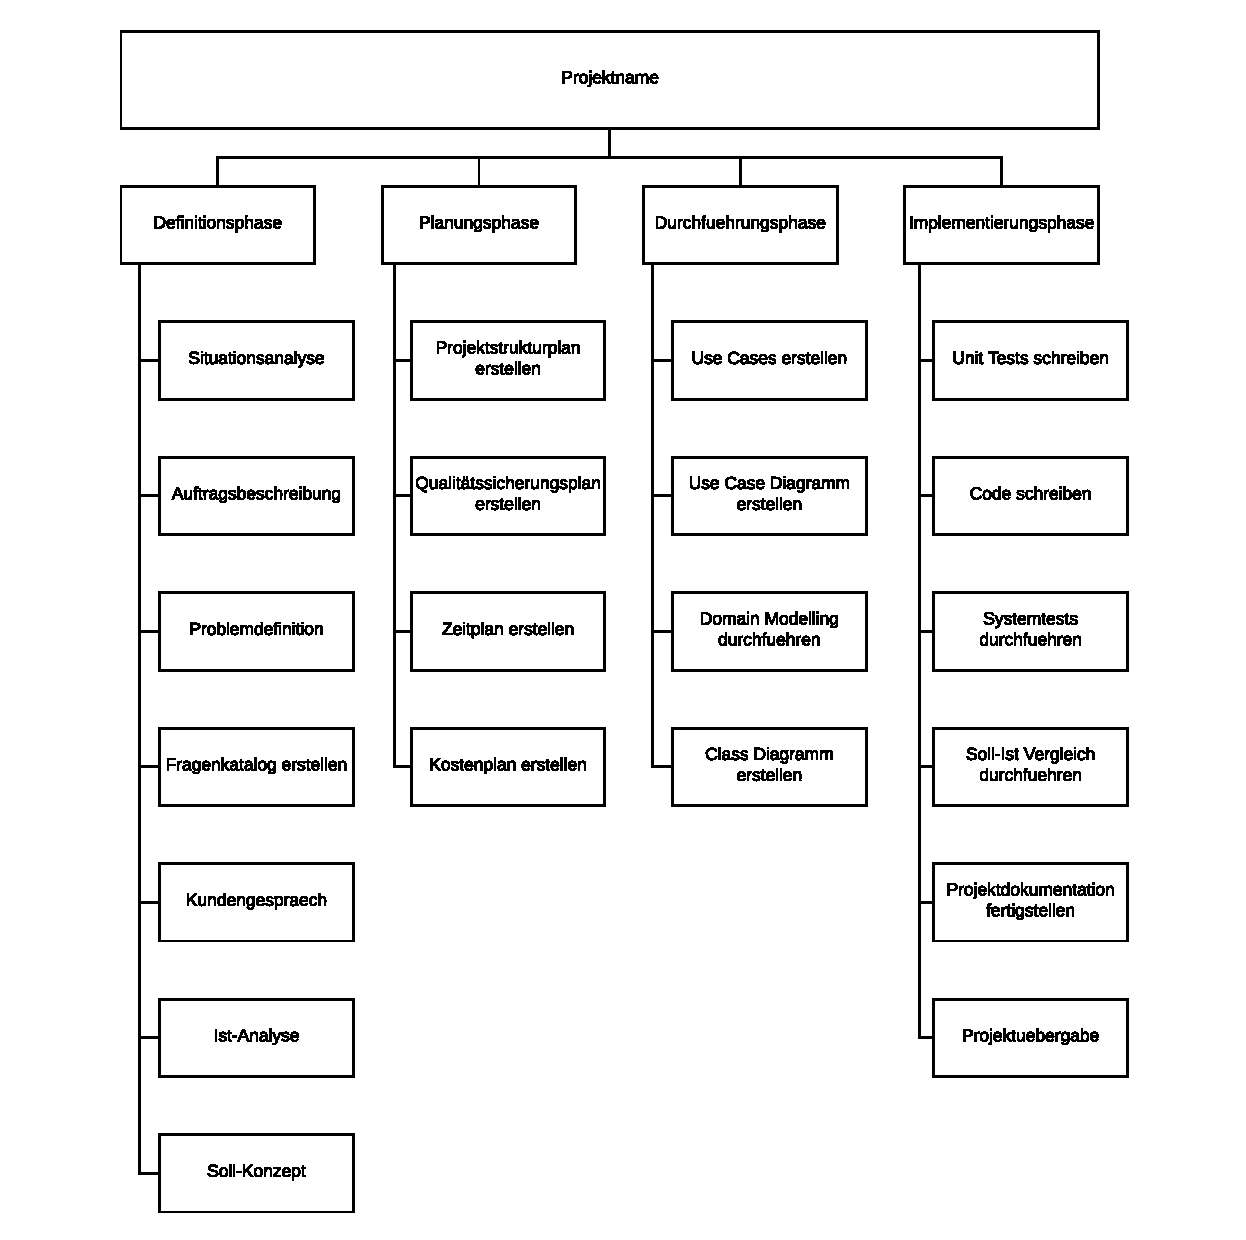
\includegraphics[width=\linewidth]{fig/Projektstrukturplan.pdf}
        \caption{Projektstrukturplan}
        \label{fig:psp}
      \end{figure}
      \newpage
    \subsection{Zeitplan}
      \newpage
    \subsection{Kostenplan}
      \newpage
    \subsection{Qualitaetssicherungsplan}
      \newpage
    \subsection{Use-Case Diagramm}
      \newpage
    \subsection{Klassendiagramm}
      \begin{figure}[h!]
        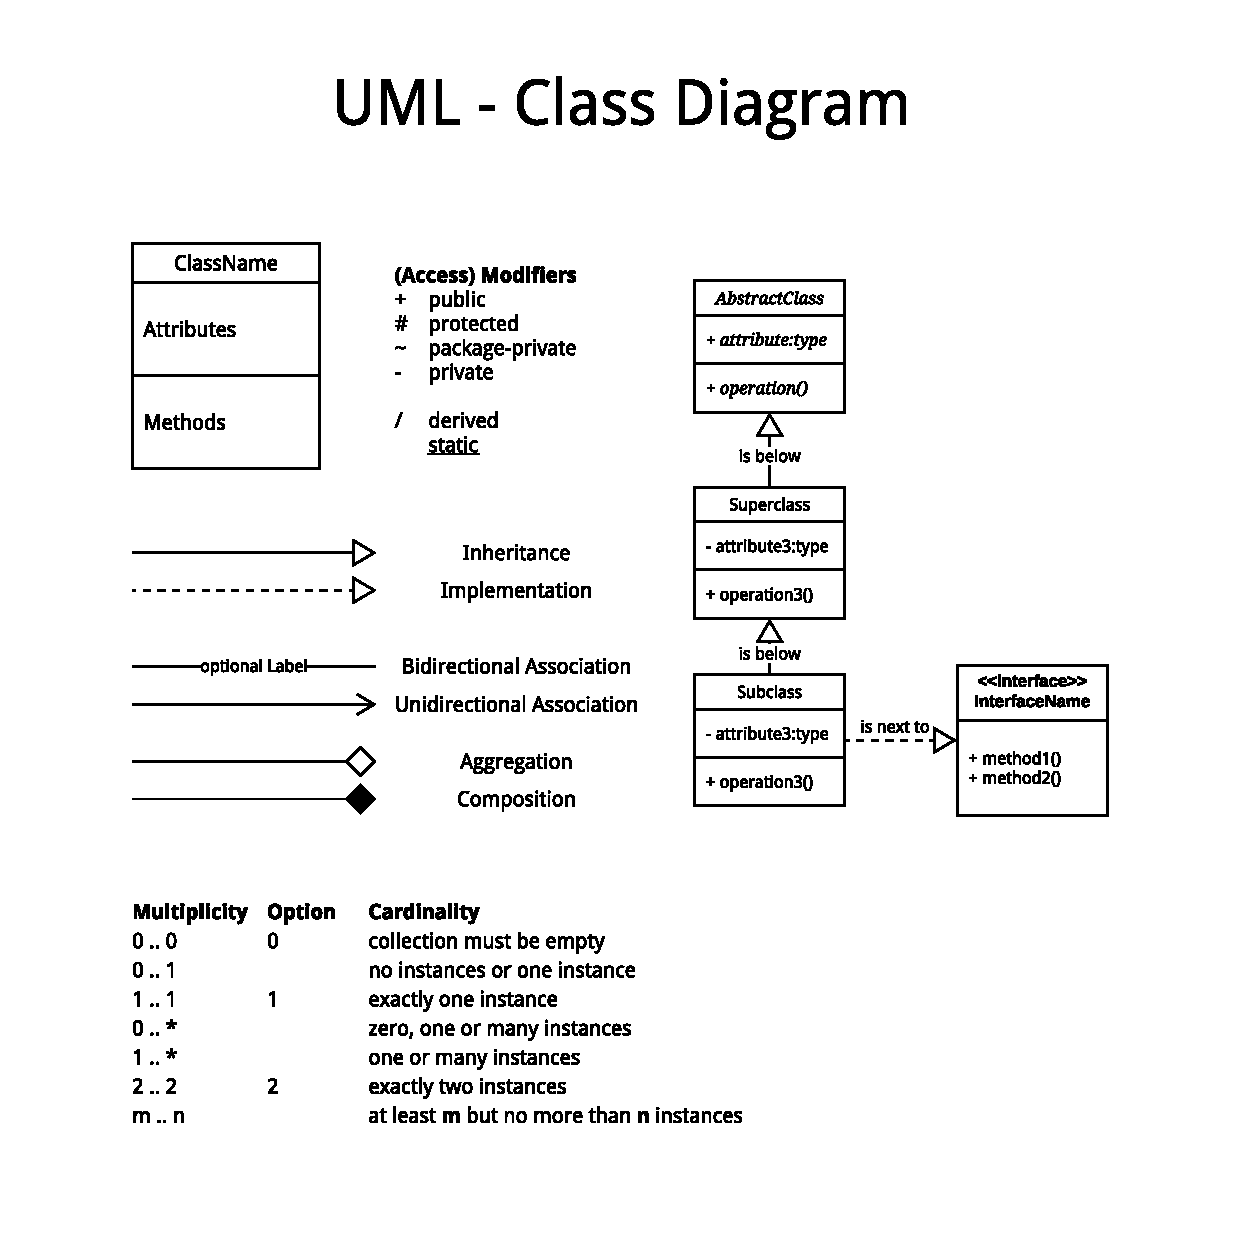
\includegraphics[width=\linewidth]{fig/UML_Classdiagram.pdf}
        \caption{Klassendiagramm}
        \label{fig:classdiagram}
      \end{figure}
      \newpage
    \subsection{Entity Relationship Diagram, Datenbank}
      \begin{figure}[h!]
        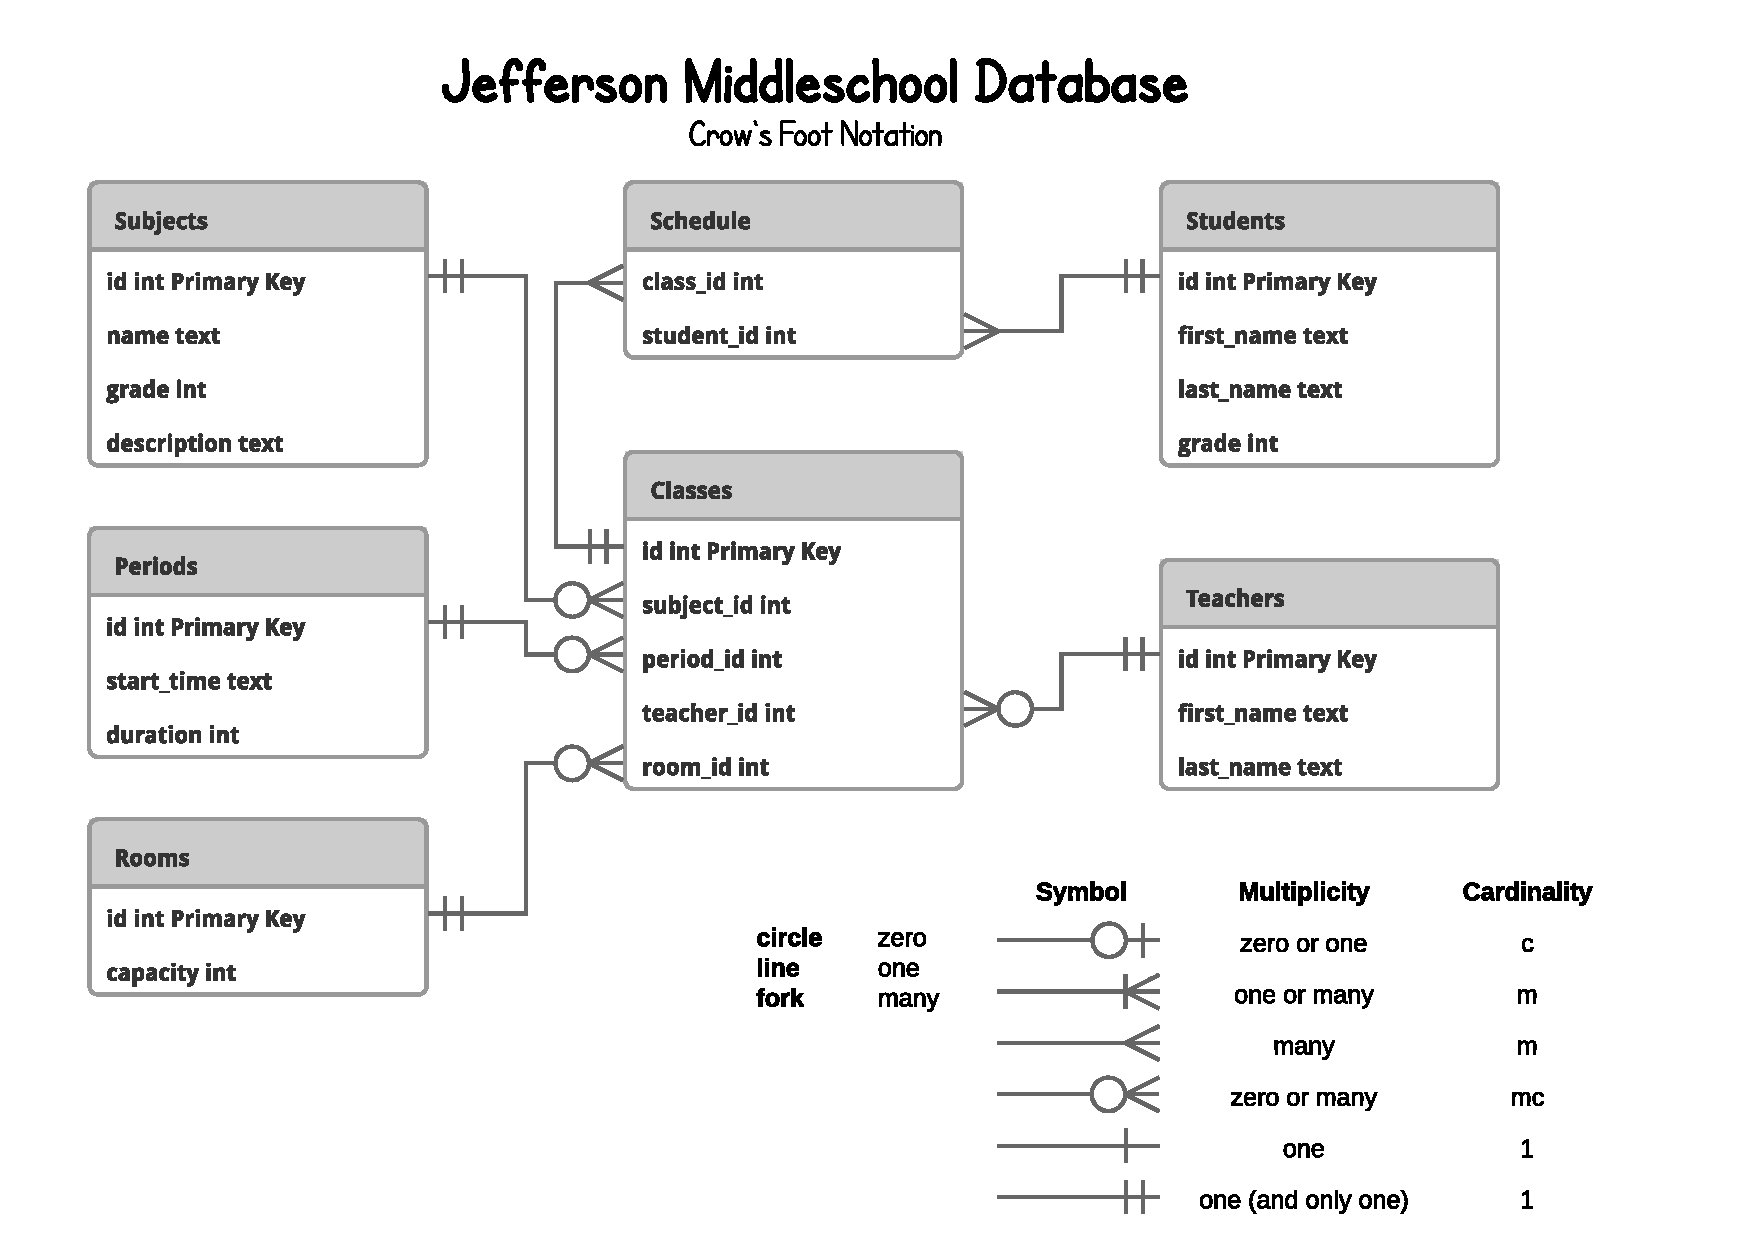
\includegraphics[width=\linewidth]{fig/ERD_JeffersonMiddleSchool.pdf}
        \caption{Entity Relationship Diagram, Datenbank}
        \label{fig:classdiagram}
      \end{figure}
      \newpage

\end{document}
